\documentclass{article}
\usepackage{lipsum}
\usepackage{enumerate}
\usepackage{amsmath, amssymb, amsthm, amsfonts}
\usepackage{url}
\usepackage{fullpage}
\usepackage{graphicx}
\usepackage[backref]{hyperref}
\usepackage{fancyvrb}
\usepackage{framed}
\usepackage{xcolor}

\definecolor{mygray}{RGB}{240,240,240}

\renewenvironment{quote}{%
  \def\FrameCommand{{\color{mygray}\vrule width 3pt}\hspace{10pt}}%
  \MakeFramed {\advance\hsize-\width \FrameRestore}}%
{\endMakeFramed}

\newtheorem{theorem}{Theorem}
\newtheorem{lemma}{Lemma}
\newtheorem{corollary}{Corollary}
\newtheorem{definition}{Definition}
\newtheorem{proposition}{Proposition}
\newtheorem{procedure}{Procedure}
\newtheorem{construction}{Construction}
\newtheorem{example}{Example}
\newtheorem{remark}{Remark}
\newtheorem{claim}{Claim}

\newcommand{\Rea}{{\mathbb R}}
\newcommand{\Int}{{\mathbb Z}}
\newcommand{\Rat}{{\mathbb Q}}
\newcommand{\Cmp}{{\mathbb C}}
\newcommand{\Nat}{{\mathbb N}}

\setlength{\oddsidemargin}{.25in}
\setlength{\evensidemargin}{.25in}
\setlength{\textwidth}{6.25in}
\setlength{\topmargin}{-0.0in}
\setlength{\textheight}{8.9in}

\renewenvironment{proof}{\noindent{\bf Proof:} \hspace*{1mm}}{
	\hspace*{\fill} $\Box$ }
\newenvironment{proof_of}[1]{\noindent {\bf Proof of #1:}
	\hspace*{1mm}}{\hspace*{\fill} $\Box$ }
\newenvironment{proof_claim}{\begin{quotation} \noindent}{
	\hspace*{\fill} $\diamond$ \end{quotation}}

\newcommand{\handout}[6]{
   \renewcommand{\thepage}{#1-\arabic{page}}
   \noindent
   \begin{center}
   \framebox{
      \vbox{
    \hbox to 5.78in { {\bf #2} \hfill #3 }
       \vspace{4mm}
       \hbox to 5.78in { {\Large \hfill #4  \hfill} }
       \vspace{2mm}
       \hbox to 5.78in { {\it #5 \hfill #6} }
      }
   }
   \end{center}
   \vspace*{4mm}
}
\newcommand{\lecture}[3]{\handout{#1}{Algorithmic Game Theory, 2023 Spring}{#2}{Homework #1}{Lecturer: Zhengyang Liu}{Student: #3}}

\begin{document}

%header --- replace with appropriate values
\lecture{2}{\today}{1120212477 \; Linkang Dong}

\tableofcontents

\section{Problem 1: My favourite result and the reason}
$\quad\;$
My favorite result in our class is the Arrow-Debreu-McKenzie Theorem. 

When I meet this theorem, I am curious about the reason of existence of competitive market equilibrium. I have learned that the existence of competitive market equilibrium is a fundamental result in economics, and it is also a key result in general equilibrium theory. However, I have not learned the rigorous proof of the existence of competitive market equilibrium. Therefore, I search the theory of general equilibrium on the Internet. Then I find that the proof of this theorem is very hard for me to understand the proof. However, I still think this theorem is very important for economics and it is also very important for our class. Therefore, I think this theorem is my favorite result in our class. Here I want to use the wikipedia to introduce this theorem and my understanding of this theorem.

In mathematical economics, the Arrow-Debreu model is a theoretical general equilibrium model. It posits that under certain economic assumptions (convex preferences, perfect competition, and demand independence) there must be a set of prices such that aggregate supplies will equal aggregate demands for every commodity in the economy.The A-D model is one of \textbf{the most general models} of competitive economy and is a crucial part of general equilibrium theory, and it can be used to prove \textbf{the existence of general equilibrium} (or Walrasian equilibrium) of an economy. In general, there may be many equilibria.\cite{wiki:Arrow-Debreu_model}

From my perspective, this theorem has significant implications for economics. It highlights the efficiency of competitive markets, where no agent can be made better off without making another agent worse off(Pareto optimality). The theorem also provides a relatively rigorous foundation for understanding competitive economy and the efficiency of resource allocation. I remember that there is a famous saying in economics: “There is no free lunch”. This theorem also reflects this saying. In a competitive market, the price of a commodity is determined by the market supply and demand. If the price of a commodity is lower than the market price, the demand for the commodity will increase, and the supply of the commodity will decrease. The price of a commodity will rise until the supply and demand of the commodity reach a balance. Therefore, the price of a commodity is determined by the market supply and demand, and the price of a commodity is the most reasonable price and there is no free lunch in the market. In some degree, the stability of the commodity's price also means that people's preferences, business competition, demand independence, etc. force the market to reach equilibrium.

I think its implications can extend to various areas of economics, making it a key result that contributes to our understanding of market mechanisms and welfare economics.

\section{Problem 2: Prove something}

\subsection{Problem} (4pt per question) Given a set function v : $2^M \rightarrow \mathbb{R}_{\ge 0}$, and for any subsets $S, T \subseteq M$ we have that
\[
   v(S) + v(T) \ge v(S \cap T) + v(S \cup T)  .
\]
For simplicity, we abuse notations $S \cup {j}$ as $S + j$ and $S~ \backslash~\{j\}$ as $S - j$, for any $j \in M$.

\begin{enumerate}
   \item Prove that for any $S \subseteq T \subseteq M$, we have 
   
\[
  \frac{v(T+j)}{v(T)} \le \frac{v(S+j)}{v(S)}. 
\]
   \item Prove that for any $T \subseteq M$ we have
   
\[
   v(T) \ge \sum_{k \in T} [v(T) - v(T-k)].
\]

\textit{Notes: the set function is default to be monotone and $v(\emptyset) = 0$ (Our Lecturer has mentioned this in the Dingding Group).}

\end{enumerate}

\subsection{Proof}

\begin{enumerate}
   \item \textbf{Proof:}
   For the set function $v$ is monotone and $v(\emptyset) = 0$ , we can easily get the following conclusion:

   \begin{itemize}
      \item $ v(S) \ge 0, v(\emptyset) = 0 \Rightarrow v(S) \ge v(\emptyset)$
      \item $ v(S) \le v(S + j) $
      \item $S \subseteq T \Rightarrow v(S) \le v(T)$ 
   \end{itemize}

   Let's consider the set $S$ and its superset $T$,where $S \subseteq T \subseteq M$. According to the condition of the problem(For any subsets $S, T \subseteq M$, $v(S) + v(T) \ge v(S \cap T) + v(S \cup T)$), For any $j \in M$, we discuss the following three cases of $j$:

   % \begin{enumerate}
   %    \item $v(X) + v(j) \ge v(X + j),\text{where } X \subseteq M\quad \text{(1)}$\\
   %    The proof is simple:
   %    \begin{itemize}
   %       \item Let $S = \{j\}$, and $T = X$  : $v(X) + v(j) \ge v(X \cap \{j\}) + v(X \cup \{j\}) $
   %       \item if $j \in X$, then $v(X \cap \{j\}) = v(\{j\}) $ and $v(X \cup \{j\}) = v(X)$, so that the formula above will be like this, $v(X) + v(j) \ge v(j) + v(X) $, which is obviously true
         
   %       \item if $j \notin X $, then $v(X \cap \{j\}) = v(\emptyset) = 0 $ and $v(X \cup \{j\}) = v(X + j)$, so that the formula above will be like this, $v(X) + v(j) \ge v(X + j) $, here $j \in X $ is also fit this formula because $v(j) \ge 0 $
   %    \end{itemize}
   %    \item According to (1), we can get:
   %    \[
   %       v(S) + v(j) \ge v(S + j) \quad \text{(2)}
   %    \]
      
   %    \[
   %       v(T) + v(j) \ge v(T + j) \quad \text{(3)}
   %    \]

   % \end{enumerate}

   % Now, let's minus inequality (3) both sides by $v(S)$:
   
   % \[
   %    v(T) + v(j) - v(S) \ge v(T + j) - v(S)
   % \]

   % \[
   %       \Rightarrow v(T)  - v(S) \ge v(T + j) - v(S) -  v(j)   
   % \]

   \begin{figure}[htbp]
      \centering
      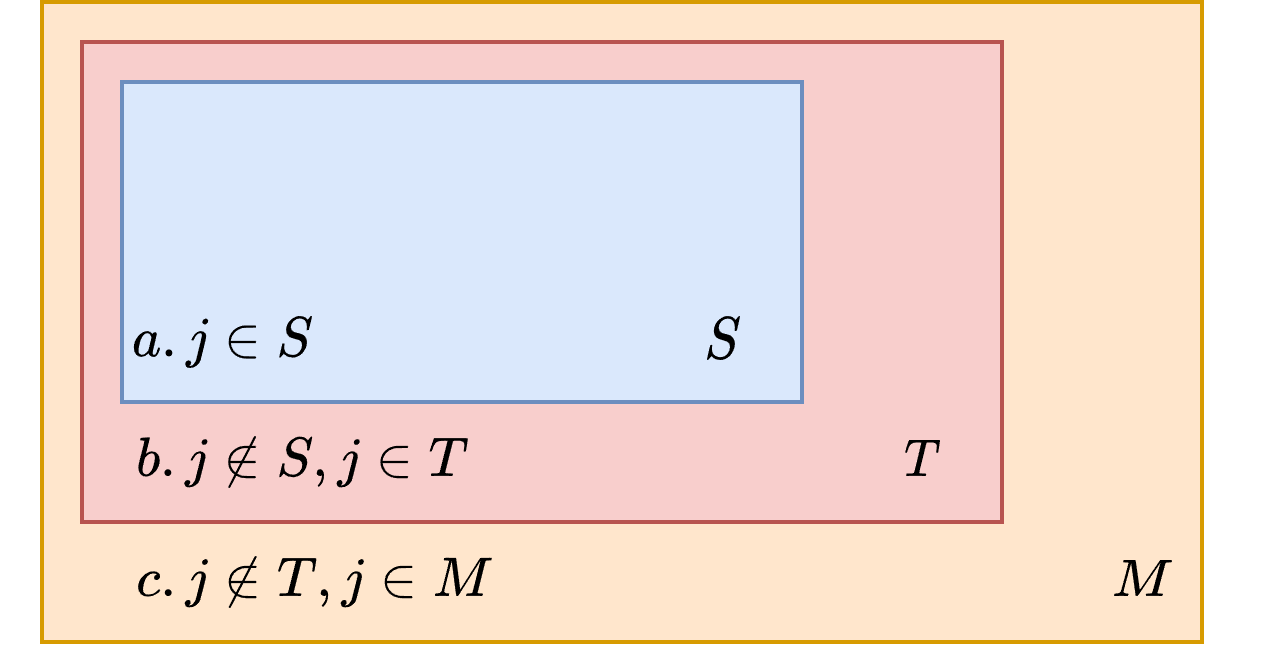
\includegraphics[width=0.5\textwidth]{image/cases.png}
      \caption{Three cases of j}
      \label{fig:example}
    \end{figure}
   
   \begin{enumerate}
      \item $j \in S$ : 
      
      In this case, we have:
      \[
         j \in S , S \subseteq T \Rightarrow j \in T
      \]
      \[
         S \cup \{j\} = S, T \cup \{j\} = T \Rightarrow v(T+j) = v(T), v(S+j) = v(S)
      \]
      Using the result above can prove our problem easily: 
      \[
         \frac{v(T+j)}{v(T)} = 1 = \frac{v(S+j)}{v(S)}
      \]
      \item $j \notin S, j \in T$ :
      
      We have:
      \[
         \frac{v(T+j)}{v(T)} = 1
      \]

      Knowing that $ v(S) \le v(S + j) $ , we have:

      \[
         \frac{v(S+j)}{v(S)} \ge 1
      \]

      Using the result above can prove our problem easily: 
      \[
         \frac{v(T+j)}{v(T)} = 1 \le \frac{v(S+j)}{v(S)}
      \]


      \item $j \notin T, j \in M$ :
      
      Knowing that for any subsets $S, T \subseteq M$, $v(S) + v(T) \ge v(S \cap T) + v(S \cup T)$, here we replace the $S$ to $S+j$ and simplify the formula:

      \[
         v(S+j) + v(T) \ge v((S\cup j) \cap T) + v((S\cup j) \cup T)
      \]

      We know that $(S\cup j) \cap T = (S \cap T) \cup (j \cap T) = S \cup \emptyset = S$, and $(S\cup j) \cup T = (S \cup T) \cup j = T \cup j$, so the formula above can change to this:
      \[
         v(S+j) + v(T) \ge v(S) + v(T+j)
      \]
      Rearranging the terms, we have:
      \[v(T+j) - v(T) \le v(S+j) - v(S)\]

      Dividing both sides by $v(T)$ and $v(S)$ (which are non-negative, and $v(T) \ge v(S)$) and rearranging the terms, we obtain:
   
      \[
         \frac{v(T+j)}{v(T)} \le \frac{v(S+j)}{v(S)}
      \]

   \end{enumerate}

   Therefore, the statement holds for any $S \subseteq T \subseteq M$.
   
   
   
   

   \item \textbf{Proof:}
   Let's consider a set $T$ and an element $k \in T$. We can rewrite $T-k$ as $T \backslash \{k\}$. We assume that $ T = \{ k_1, k_2, ..., k_n \} $, where $k_i$ is the $i$th element in the set $T$ and $n$ is the number of elements in the set $T$. And we know the element $k \in \{ k_1, k_2, ..., k_n \}$.
   The set function satisfies the inequality property which is mentioned in the problem, so we have:
   
   \[
      v(T ) + v(T - \{k\}) \ge v(T \cap (T - \{k\})) + v(T \cup (T - \{k\}))
   \]
   
   Notice that $T \cap (T - \{k\}) = T - \{k\} $ and $T \cup (T - \{k\}) = T$, and we have the following formula which obviously holds:
   
   \[
      v(T ) + v(T - \{k\}) \ge v(T - \{k\}) + v(T)   
   \]
   
   
   Now, let's think more about it, let the set $S$ be $T - \{k_1\}$ and $T - \{k_2\}$, and we have:

   \[
      v(T - \{k_1\}) + v(T - \{k_2\}) \ge v((T - \{k_1\}) \cap (T - \{k_2\})) + v((T - \{k_1\}) \cup (T - \{k_2\}))
   \]
   
   Easily knowing that $(T - \{k_1\}) \cap (T - \{k_2\}) = T - \{k_1\} - \{k_2\} = T - \{k_1, k_2\}$ and $(T - \{k_1\}) \cup (T - \{k_2\}) = T$, so we have:

   \[
      v(T - \{k_1\}) + v(T - \{k_2\}) \ge v(T - \{k_1, k_2\}) + v(T) \quad \text{ (1) }
   \]

   And we want to construct the symbol $\sum$, so we let the input of the inequality be $T - \{k_1,k_2\}$ and $T - \{k_3\}$, and we have:

   \[
      v(T - \{k_1,k_2\}) + v(T - \{k_3\}) \ge v(T - \{k_1,k_2,k_3\}) + v(T) \quad \text{ (2) }
   \]

   Plusing inequality (1) with $v(T - \{k_3\})$ both sides and using the inequality (2) above, we have:

   \[
      v(T - \{k_1\}) + v(T - \{k_2\}) + v(T - \{k_3\}) \ge v(T - \{k_1,k_2,k_3\}) + 2 * v(T)
   \]

   Following this rule, we can construct the symbol $\sum$ to make the inequality more general, so we have:

   \[
      \sum_{k \in T} v(T - \{k\}) \ge v(T - \{k_1,\ldots,k_n\}) + (n-1) * v(T)
   \]

   Knowing that $T - \{k_1,\ldots,k_n\} = \emptyset$, so we have:

   \[
      \sum_{k \in T} v(T - \{k\}) \ge (n-1) * v(T)
   \]

   Plusing $v(T)$ both sides, we have:

   \[
      \sum_{k \in T} v(T - \{k\}) + v(T) \ge n * v(T)
   \]
   

   By rearranging terms, we get:
   
   \[
     v(T) \ge \sum_{k \in T}[v(T) - v(T - \{k\})]
   \]
   
   Therefore, the statement holds for any $T \subseteq M$.

\end{enumerate}


\section{Problem 3: EFX always exists}

\begin{enumerate}
   \item (3pt) Show that EFX always exists for identical valuations.
   \item (2pt) Show that EFX always exists when n = 2. (Hint: you can use the first result.)
\end{enumerate}

\paragraph{Problem 1:}
To show that EFX (Envy-Free Allocation with Indivisible Goods) always exists for identical valuations, we need to demonstrate that there exists an allocation of goods to the agents such that no agent envies another agent.

Let's consider a scenario with identical valuations, where all agents have the same valuation function v, $2^m \rightarrow \mathbb{R}$, $v(S)$ for any subset of goods $S$. In such a case, the goods are equally valuable to all agents(Because all agents have the same valuation function). 

Now, let's \textbf{distribute the goods equally} among the agents. Since all agents have identical valuations, they will value the goods equally as well. Therefore, no agent will envy another agent because they all receive the same allocation of goods.

Thus, EFX always exists for identical valuations.

\paragraph{Problem 2:}
Now, we need to show that EFX always exists when $n=2$ (i.e., there are two agents). We can use the result from Problem 1 to prove this.

In the case of two agents, we can also assume that both agents have identical valuations. According to the result from Problem 1, EFX exists for identical valuations. Therefore, there exists an envy-free allocation of goods such that both agents value their allocated goods equally and do not envy each other.

Thus, EFX always exists when $n=2$. 

(However, it requires exponentially many queries to compute the EFX.\cite{DBLP:journals/corr/PlautR17} The description of the orginal paper is as follows.)

\begin{quote}
   By identical valuations, all players have the same
valuation. This result also yields a cut-and-choose-based protocol for two players with general and possibly distinct valuations that is guaranteed to produce an EFX allocation. This is consistent
with our exponential lower bound, as it is well known that finding the leximin solution can require exponential time for general valuations.
\end{quote}

\section{Problem 4: XOS function}

\subsection{Problem}(5pt) Given a valuation function v : $2^{[m]} \rightarrow \mathbb{R}$ which is normalized (i.e., $v(\emptyset) = 0$) and
monotone (i.e., $v(S) \le v(T)$ once $S \subseteq T \subseteq [m]$). $v$ is additive iff $v(S) = \sum_{i \in S} v(i)$ for any $S \subseteq [m]$. $v$ is submodular iff $v(S \cup T) + v(S \cap T) \le v(S) + v(T)$ for any $S, T \subseteq [m]$. And $v$ is XOS iff there exist t additive valuations $\{a_1, . . . , a_t\}$ such that $v(S) = max_{r \in [t]} a_r(S)$ for every $S \subseteq [m]$.

Prove that any monotone and normalized submodular function can be written as an XOS function.

\subsection{Proof}

From the problem description of XOS and the additive concept , we have the following definition of XOS function:

\begin{definition}
   A valuation function $v : 2^{[m]} \rightarrow \mathbb{R}$ is XOS iff there exist t additive valuations $\{a_1, . . . , a_t\}$ such that $v(S) = max_{r \in [t]} a_r(S)$ for every $S \subseteq [m]$.
\end{definition}

Polishing the definition by replacing additive valuations $a_r$ with $v$, we have:

\begin{definition}
   A valuation function $v : 2^{[m]} \rightarrow \mathbb{R}$ is XOS iff we can write it as $v(A) = max_{k}\sum_{j \in A} v^k_j$ for every $A \subseteq [m]$.  For valuations on using item j in a specific way $k$, $v^k_j$. Note that this is not exponentiating $v_j$ but rather indexing into the valuations with a particular usage $k$(order).
\end{definition}

After recalling the definition of XOS, We now prove this by showing that a monotone and normalized submodular valuation function V must be XOS.

Assume we have some ordering of the items. Let's call this $\pi$. Now, we define:

\[
  S^{\pi}_j = \{i \in [m] : \pi(i) \le \pi(j)\}
\]

To understand this, we can see that $S^{\pi}_j$ is the set of items that are ordered before or at the same time as item j. For instance, $S = \{a,b,c,d,\ldots,z\}$, but ordering $\pi$ is $\{a, b, c, d, e, q, z, j, y\}$, then $S^{\pi}_{<j} = \{a, b, c, d, e, q, z\}$ and $S^{\pi}_{j} = \{a, b, c, d, e, q, z, j\}$. 

Furthermore, we can use the definition of submodularity combined with an ordering $\pi$ to build a value function $V^{\pi}_j$ iteratively:

\[
  V^{\pi}_j = V(S^{\pi}_j) - V(S^{\pi}_{j-1})
\]

$V^{\pi}_j$ is the value of item j in ordering $\pi$. For the reason of building $V^{\pi}_j$ iteratively, we can remember the decreasing marginal utility property of submodular function(we have prove this in Problem 2), for any $S \subseteq T \subseteq [m]$:

\[v(T+j) - v(T) \le v(S+j) - v(S)\]

Knowing that $S^{\pi}_j$ is the set of items that are ordered before or at the same time as item j, we can see that $S^{\pi}_{j-1}$(or $S^{\pi}_{<j}$) is the set of items that are ordered before item j. In other word, $S^{\pi}_{j} = S^{\pi}_{j-1} \cup \{j\} = S^{\pi}_{j-1} + j$. Therefore, $S^{\pi}_{j-1} \subseteq S^{\pi}_j$. 

Suppose we have  $S = \{s_1,s_2,s_3,\ldots,s_n\}$ , and knowing  $V(S^{\pi}_0) = V(\emptyset) = 0$ and let $V(S) = V(S^{\pi}_n)$, 
then we have:

\begin{equation}
   \begin{aligned}
      \sum_{i\in S} V^{\pi}_i  &= \sum_{i\in S} (V(S^{\pi}_i) - V(S^{\pi}_{i-1})) \\
           &= V(S^{\pi}_1) - V(S^{\pi}_{0}) + V(S^{\pi}_2) - V(S^{\pi}_{1}) + \ldots + V(S^{\pi}_n) - V(S^{\pi}_{n-1}) \\
           &= V(S^{\pi}_n) - V(S^{\pi}_{0}) \\
           &= V(S^{\pi}_n) \\
           &= V(S)
   \end{aligned}
   \label{eq:1}
\end{equation}

Now, we take the approach of constructing some $\pi$ such that $V(S) = \sum_{i\in S} V^{\pi}_i$ for any $S \subseteq [m]$. Note that $V^{\pi}_i$ is the value of item i in ordering $\pi$. Therefore, $V(S) = \sum_{i\in S} V^{\pi}_i$ is the value of set S in ordering $\pi$. So we have:

\[
   V(S) = \sum_{i\in S} V^{\pi}_i
\]

Naturaly, we can see that the value of $V(S)$ is defined by the ordering $\pi$. So we can construct $\pi$ such that $V(S) = \max_{\pi}\sum_{i\in S} V^{\pi}_i$ for any $S \subseteq [m]$. According to the definition of XOS, we can see that $V$ is XOS because there exists t additive valuations $\{V^{\pi}_1, V^{\pi}_2, \ldots, V^{\pi}_t\}$ such that $V(S) = \max_{\pi}\sum_{i\in S} V^{\pi}_i$ for any $S \subseteq [m]$.(Note that we have given the approach of additive-valuations construction in these paragraph above.)

Now, we have proved that any monotone and normalized submodular function can be written as an XOS function.

\newpage

\bibliographystyle{plain}
\bibliography{bibliography.bib}
\end{document}